\documentclass[a4paper,12pt]{article}

\usepackage[utf8x]{inputenc}
\usepackage[english, russian]{babel}

\usepackage{tabularx}
\usepackage{multirow}
\usepackage{graphicx}
\usepackage{misccorr}
\usepackage{indentfirst}


\usepackage{listings}
\usepackage{xcolor}

\usepackage{fullpage}

\usepackage[labelsep=endash,
		    margin=10pt, 
		    justification = centerlast, 
		    format = hang,
		    singlelinecheck=false
		    ]{caption}

\exhyphenpenalty=10000
\doublehyphendemerits=10000
\finalhyphendemerits=5000

\definecolor{codegreen}{rgb}{0,0.6,0}
\definecolor{codegray}{rgb}{0.5,0.5,0.5}
\definecolor{codepurple}{rgb}{0.58,0,0.82}
\definecolor{backcolour}{rgb}{0.95,0.95,0.92}
 
\lstdefinestyle{mystyle}{
    backgroundcolor=\color{backcolour},
    commentstyle=\color{codegreen},
    keywordstyle=\color{blue},
    numberstyle=\tiny\color{codegray},
    stringstyle=\color{codepurple},
    basicstyle=\footnotesize,
    breakatwhitespace=false,
    breaklines=true,
    captionpos=t,
    keepspaces=true,
    numbers=left,
    numbersep=5pt,
    showspaces=false,
    showstringspaces=false
    showtabs=false,
    tabsize=4,
    frame=tb
}
 
\lstset{style=mystyle}

\usepackage{color}
\usepackage{xcolor}
\usepackage{listings}
 
% Цвета для кода
 
\definecolor{string}{HTML}{B40000} % цвет строк в коде
\definecolor{comment}{HTML}{008000} % цвет комментариев в коде
\definecolor{keyword}{HTML}{1A00FF} % цвет ключевых слов в коде
\definecolor{morecomment}{HTML}{8000FF} % цвет include и других элементов в коде
\definecolor{сaptiontext}{HTML}{FFFFFF} % цвет текста заголовка в коде
\definecolor{сaptionbk}{HTML}{999999} % цвет фона заголовка в коде
\definecolor{bk}{HTML}{FFFFFF} % цвет фона в коде
\definecolor{frame}{HTML}{999999} % цвет рамки в коде
\definecolor{brackets}{HTML}{B40000} % цвет скобок в коде
 

%%% Отображение кода %%%
 
% Настройки отображения кода
 
\lstset{
	%morekeywords={*,...}, % если хотите добавить ключевые слова, то добавляйте	 
	% Настройки отображения     
	breaklines=true, % Перенос длинных строк
	% Для отображения русского языка
	extendedchars=true,
	literate={Ö}{{\"O}}1
	{Ä}{{\"A}}1
	{Ü}{{\"U}}1
	{ß}{{\ss}}1
	{ü}{{\"u}}1
	{ä}{{\"a}}1
	{ö}{{\"o}}1
	{~}{{\textasciitilde}}1
	{а}{{\selectfont\char224}}1
	{б}{{\selectfont\char225}}1
	{в}{{\selectfont\char226}}1
	{г}{{\selectfont\char227}}1
	{д}{{\selectfont\char228}}1
	{е}{{\selectfont\char229}}1
	{ё}{{\"e}}1
	{ж}{{\selectfont\char230}}1
	{з}{{\selectfont\char231}}1
	{и}{{\selectfont\char232}}1
	{й}{{\selectfont\char233}}1
	{к}{{\selectfont\char234}}1
	{л}{{\selectfont\char235}}1
	{м}{{\selectfont\char236}}1
	{н}{{\selectfont\char237}}1
	{о}{{\selectfont\char238}}1
	{п}{{\selectfont\char239}}1
	{р}{{\selectfont\char240}}1
	{с}{{\selectfont\char241}}1
	{т}{{\selectfont\char242}}1
	{у}{{\selectfont\char243}}1
	{ф}{{\selectfont\char244}}1
	{х}{{\selectfont\char245}}1
	{ц}{{\selectfont\char246}}1
	{ч}{{\selectfont\char247}}1
	{ш}{{\selectfont\char248}}1
	{щ}{{\selectfont\char249}}1
	{ъ}{{\selectfont\char250}}1
	{ы}{{\selectfont\char251}}1
	{ь}{{\selectfont\char252}}1
	{э}{{\selectfont\char253}}1
	{ю}{{\selectfont\char254}}1
	{я}{{\selectfont\char255}}1
	{А}{{\selectfont\char192}}1
	{Б}{{\selectfont\char193}}1
	{В}{{\selectfont\char194}}1
	{Г}{{\selectfont\char195}}1
	{Д}{{\selectfont\char196}}1
	{Е}{{\selectfont\char197}}1
	{Ё}{{\"E}}1
	{Ж}{{\selectfont\char198}}1
	{З}{{\selectfont\char199}}1
	{И}{{\selectfont\char200}}1
	{Й}{{\selectfont\char201}}1
	{К}{{\selectfont\char202}}1
	{Л}{{\selectfont\char203}}1
	{М}{{\selectfont\char204}}1
	{Н}{{\selectfont\char205}}1
	{О}{{\selectfont\char206}}1
	{П}{{\selectfont\char207}}1
	{Р}{{\selectfont\char208}}1
	{С}{{\selectfont\char209}}1
	{Т}{{\selectfont\char210}}1
	{У}{{\selectfont\char211}}1
	{Ф}{{\selectfont\char212}}1
	{Х}{{\selectfont\char213}}1
	{Ц}{{\selectfont\char214}}1
	{Ч}{{\selectfont\char215}}1
	{Ш}{{\selectfont\char216}}1
	{Щ}{{\selectfont\char217}}1
	{Ъ}{{\selectfont\char218}}1
	{Ы}{{\selectfont\char219}}1
	{Ь}{{\selectfont\char220}}1
	{Э}{{\selectfont\char221}}1
	{Ю}{{\selectfont\char222}}1
	{Я}{{\selectfont\char223}}1
	{і}{{\selectfont\char105}}1
	{ї}{{\selectfont\char168}}1
	{є}{{\selectfont\char185}}1
	{ґ}{{\selectfont\char160}}1
	{І}{{\selectfont\char73}}1
	{Ї}{{\selectfont\char136}}1
	{Є}{{\selectfont\char153}}1
	{Ґ}{{\selectfont\char128}}1
	{\{}{{{\color{brackets}\{}}}1 % Цвет скобок {
	{\}}{{{\color{brackets}\}}}}1 % Цвет скобок }
}
\begin{document}

\begin{titlepage}
\newpage

\

\begin{center}
	\large		
   	Министерство образования и науки Российской Федерации\\[0.5cm]
    	
	ФГБОУ ВО Рыбинский государственный авиационный технический университет имени П.А. Соловьева\\[1.0cm]

	Факультет радиоэлектроники и информатики\\[0.25cm]
		
	Кафедра математического и программного обеспечения\\ электронных вычислительных средств\\[1.5cm]
	
	\Large
	\textbf{\textsc{ОТЧЕТ ПО ЛАБОРАТОРНОЙ РАБОТЕ №3}}\\[0.25cm]
	по  дисциплине\\
	\textbf{Тестирование и отладка\\ программного обеспечения}\\[0.5cm]
	
	по теме\\
	Интеграционное тестирование
	
\end{center}

\vfill	
\begin{tabularx}{0.95\textwidth}{lXr}
Студенты группы ИПБ-13 			& &	Болотин Д. И.\\
								& &	Ивашин А.В. \\
Преподаватель к.т.н., ст. преп.	& & Воробьев К. А.\\
\end{tabularx}

\vspace{1.5cm}
\center Рыбинск 2016
\end{titlepage}	


\newpage
\setcounter{page}{2}

\tableofcontents

\newpage\section{Общее описание тестируемой системы}

Прект предназначен для шифрования/дешифрования текстов методами Моноалфавитной замены, Побитовой перестановки.
На Рисунке \ref{fig:class_diagram} представлена  диаграмма классов проекта.

\par После запуска программы пользователь видит окно авторизации (Рисунок. \ref{fig:login_form}), с помощью которого он может либо авторизаоваться: введя логин (аглийский алфавит) и пароль; зарегистрироваться (Рисунок \ref{fig:registry_form}): введя информацию о себе и выбрав предпочтительные методы шифрования - представлены на интерфейсе двумя выпадающими списками (обязательными явлюятся поля: логин, пароль и методы шифрования, если в обоих выпадающих списках выбран один и тот же метод, то в БД попадает лишь один и пользователю будет доступна работа только с одним методом); либо же завершить работы с программой с помощью кнопки "Выход".
\begin{center}
	\begin{figure}[h!]
		\centering
   		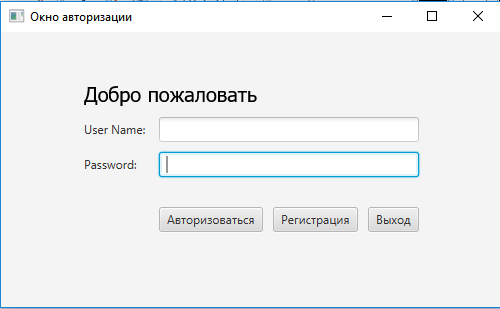
\includegraphics[scale=0.5]{img/login_form.png}
   		\caption{Окно авторизации}
   		\label{fig:login_form}
    \end{figure}
\end{center}
\begin{center}
	\begin{figure}[h!]
		\centering
   		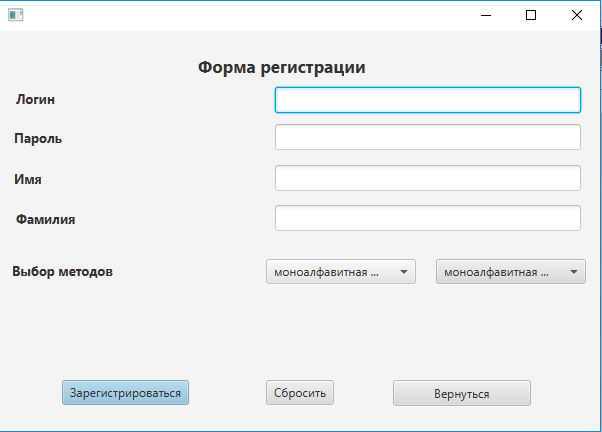
\includegraphics[scale=0.5]{img/registry_form.png}
   		\caption{Окно регистрации}
   		\label{fig:registry_form}
    \end{figure}
\end{center}
\par После прохождения авторизации пользователю открывается главное окно приложения, в котором ему, из списка методов шифрования, будут доступны лишь те методы, которые были выбраны им на этапе регистрации (Рисунок. \ref{fig:main_form}).
\begin{center}
	\begin{figure}[h!]
		\centering
   		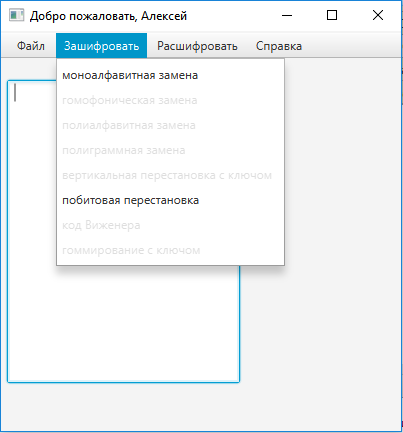
\includegraphics[scale=0.5]{img/main_form.png}
   		\caption{Главное окно программы}
   		\label{fig:main_form}
    \end{figure}
\end{center}

\begin{center}
	\begin{figure}[h!]
		\centering
   		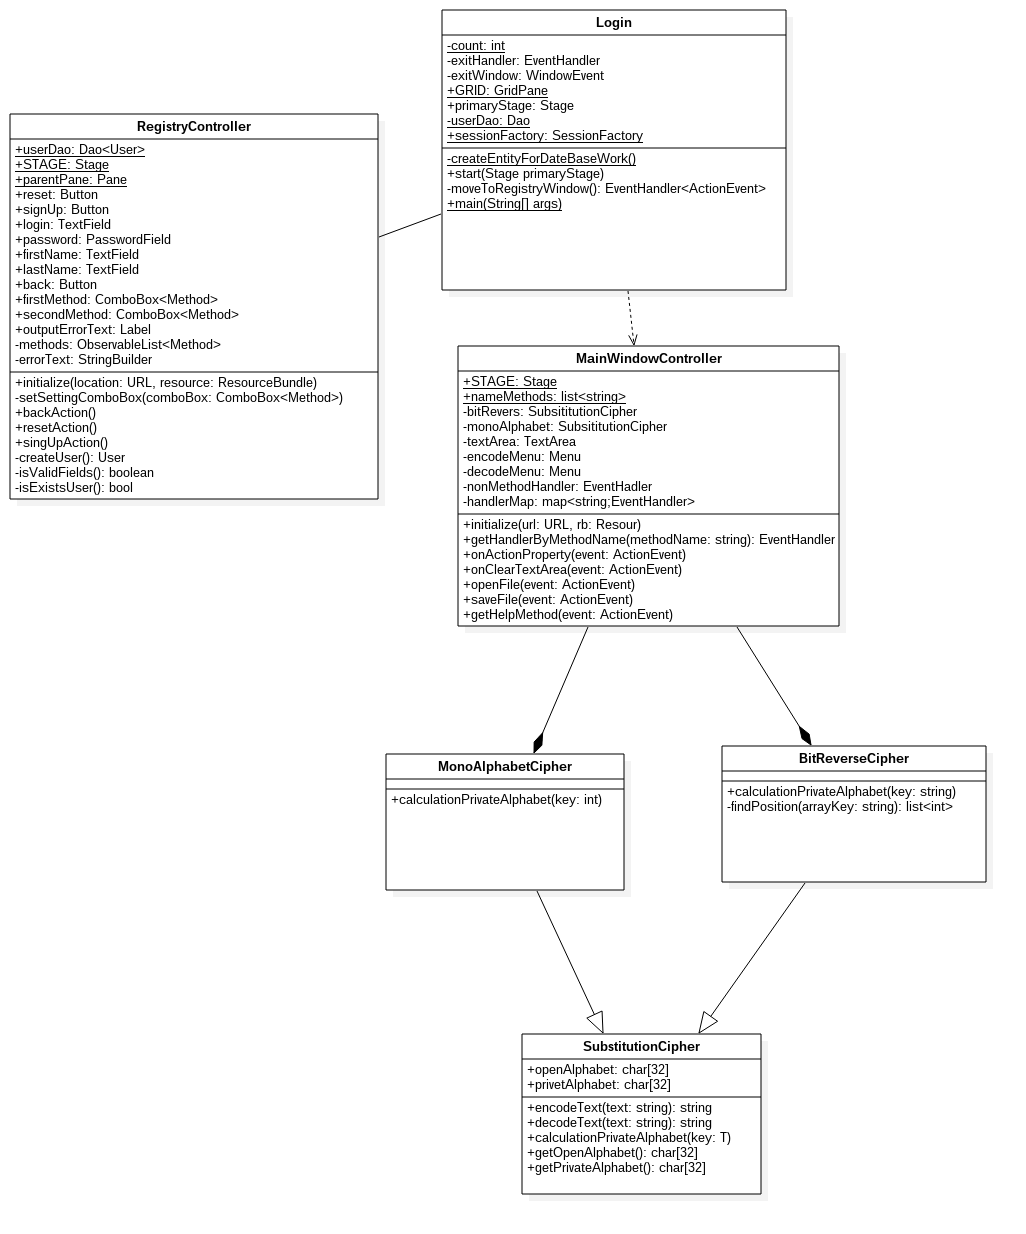
\includegraphics[scale=0.5]{img/class_diagram.png}
   		\caption{Диаграмма классов проекта}
   		\label{fig:class_diagram}
    \end{figure}
\end{center}

\newpage\section{Общее описание тестируемых классов}
В ходе данного тестирования проверяется только взаимодействие классов программы между собой, взаимодействие с другими системами не проверяется.

Тестированию подвержены классы, взаимодействующие друг с другом непосредственно, а также взаимодействие MonoAlphabetCipher и BitReversCipher посредством комбинации различных способов шифрования/дешифрования.
Тестирование добавления пользователя в БД в данной работе не производится.

Для проведения тестирования использована библиотека JUnit, а также TestFX, которая нужна для моделирования взаимодействия пользователя с интерфейсом.
\subsection{Ограничения для шифруемого/расшифруемого текста}
Текст принимаемвй методами шифрования состоит из строчных букв русского алфавита, из которого изключены буквы 'ё' и 'й', а так же пробел. Оставшиеся символы не входят в состав открытого алфавита, поэтому при их использовании их в тексте пользователь увидит следующее сообщение: "Недопустимый символ. Расшифровка/Шифрование не возможно" (Последнее предложение зависит от выбранного пользователем метода. Пример на рисунке \ref{fig:wrong_char_and_response}.
\begin{center}
	\begin{figure}[h!]
		\centering
		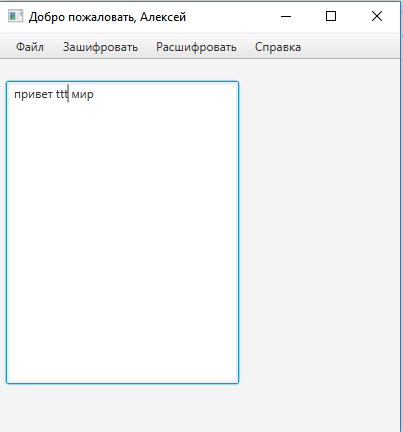
\includegraphics[scale=0.7]{img/wrong_char.png}
		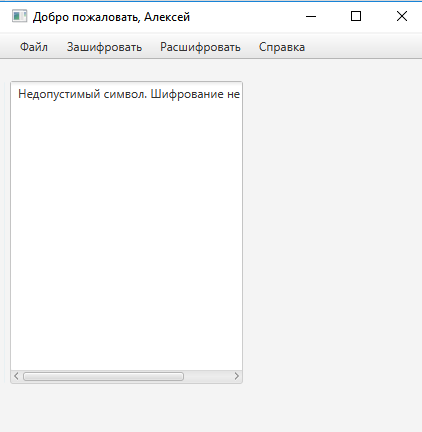
\includegraphics[scale=0.7]{img/wrong_char_response.png}
		\caption{Не верный символ в тексте}
		\label{fig:wrong_char_and_response}
	\end{figure}
\end{center}

\newpage\section{Общее описание тестирующих классов}
Для проведения интеграционного тестирования была разработана система классов для тестирования пользовательского интерфейса(т.к. почти все классы программы взаимодействуют только через него), а также класс для тестирования взаимодействия методов шифрования (под названием IntegrationCipherTest). Диаграмма классов для интеграционного тестирования пользовательского Gui представлена на рисунке \ref{fig:class_diagram_test_gui}, на ней упущены имена методов и атрибутов.
\begin{center}
	\begin{figure}[h!]
		\centering
   		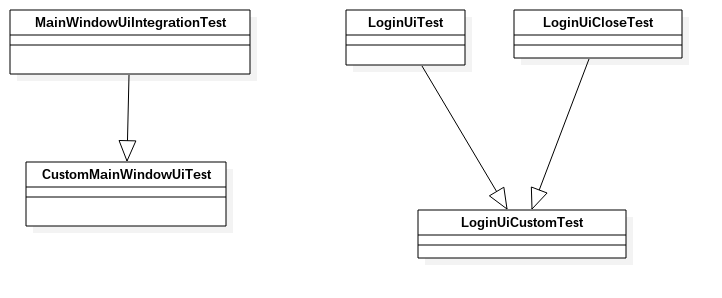
\includegraphics[scale=0.6]{img/class_diagram_testing.png}
   		\caption{Диаграмма тестирующих классов}
   		\label{fig:class_diagram_test_gui}
    \end{figure}
\end{center}


\newpage\section{Тестирование взаимодействия класса Login}
Login - это главный класс приложения, который запускает его и одновременно является контроллером для окна авторизации. Пользователь должен пройти авторизацию или зарегистрироваться. Если после третьей попытки не удалось авторизиваться, то программа закрывается.
\subsection{Закрытие программы при неверной авторизации}
С помощью TestFx моделируется попытка неудачной авторизации: три раза вводим не верный пароль. На каждом шаге проверяем появилось ли в специальной строке сообщение об ошибке: "Не верный пароль''", выделенное красным цветом. (Листинг \ref{listing_login:test_wrong_authorization}).
\begin{lstlisting}[language=java, caption=Тестирование неверной авторизации, label=listing_login:test_wrong_authorization]
public class LoginUiCloseTest extends LoginUiCustomTest {
    @Test
    public void threeWrongAuthorizationTest() {
        for (int i = 0; i < 3; i++) {
            clickOn(userName).write("Aleksey");
            clickOn(password).write("tttt");
            clickOn(authorization).sleep(100);
            verifyThat(resultAuthorization, hasText("Не верный пароль"));
            assertEquals(resultAuthorization.getFill(), Color.FIREBRICK);
            userName.clear();
            password.clear();
        }
        assertEquals(stage.isShowing(), false);
        assertEquals(sessionFactory.isClosed(), true);
    }
}
\end{lstlisting}

\subsection{Реакция программы при неверном пароле}
При вводе корректного (существующего) логина пользователя, но некорректного пароля для него в специальной строке формы авторизации должна появиться надпись "Неверный пароль''", выделенная красным цветом. Этот (Листинг \ref{listing_login:test_wrong_password}) и последующие тесты класса Login описаны в классе LoginUiTest.

\begin{lstlisting}[language=java, caption=Тестирование ввода неверного пароля, label=listing_login:test_wrong_password]      
    @Test
    public void wrongAuthorizationTest() {
        assertEquals(sessionFactory.isClosed(), false);
        clickOn(userName).write("Aleksey");
        clickOn(password).write("retdfgdfh");
        clickOn(authorization);
        verifyThat(resultAuthorization, hasText("Не верный пароль"));
        assertEquals(resultAuthorization.getFill(), Color.FIREBRICK);
    }
\end{lstlisting}

\subsection{Реакция программы при не существующем логине}
После нажатия на кнопку авторизации в БД ищется пользователь с указаным логином, если не возвращается пользователь с таким логином, то должно появиться сообщение: "Такого пользователя не существует" (Листинг \ref{listing_login:test_wrong_user}).
\begin{lstlisting}[language=java, caption=Тестирование при несуществующем логине, label=listing_login:test_wrong_user]
    @Test
    public void thisUserDoesntExistTest() {
        assertEquals(sessionFactory.isClosed(), false);
        clickOn(userName).write("ТестНик");
        clickOn(password).write("tttt");
        clickOn(authorization);
        verifyThat(resultAuthorization, hasText("Такого пользователя не существует"));
        assertEquals(resultAuthorization.getFill(), Color.FIREBRICK);
    }
\end{lstlisting}


\subsection{Реакция программы при верной авторизации}
При прохождении авторизации окно авторизации должно закрыться, а вместо него должно появиться основное окно программы (Листинг \ref{listing_login:test_true_autorization}). 

\begin{lstlisting}[language=java, caption=Тестирование прохождения авторизации, label=listing_login:test_true_autorization]
    @Test
    public void openMainWindowTest() {
        assertEquals(sessionFactory.isClosed(), false);
        clickOn(userName).write("Aleksey");
        clickOn(password).write("yui");
        clickOn(authorization);
        verifyThat(resultAuthorization, hasText("Пароль верный"));
        assertEquals(resultAuthorization.getFill(), Color.GREEN);
        waitUntil("#AnchorPane", visible());
    }
\end{lstlisting}

\subsection{Тестирование перехода к окну регистрации}
При нажатии на кнопку "'Регистация'' , должно появится соответствующее окно, а окно для авторизации исчезнуть (Листинг \ref{listing_login:test_registration_to_registration}). 
\begin{lstlisting}[language=java, caption=Тестирование перехода к окну регистрации, label=listing_login:test_registration_to_registration]
	protected void openRegistryWindowAndTest() {
        clickOn(registry);
        assertEquals(gridPane.isDisable(), true);
        waitUntil("#registryPane", visible());
    }

    protected void closeRegistryWindowAndTest() {
        clickOn("#back");
        assertEquals(gridPane.isDisable(), false);
    }     
    @Test
    public void openRegistryWindowTest() {
        openRegistryWindowAndTest();
        closeRegistryWindowAndTest();
    }
\end{lstlisting}

\newpage\section{Тестирование взаимодействия классов \\MonoAlphabetCipher и BitReverseCipher}
Тестирование осуществляется посредством многократного шифрования и расшифрования текста различными методами. После последовательного шифрования и расшифрования разными методами с неизменными ключами текст должен совпасть с исходным. Если провести такой же тест, но при расшифровании изменить ключ одного из методов, то результат должен не совпасть с исходным. Далее проведём тест, при котором зашуфруем несколько раз обоими методами с разнами ключами и расшуфруем в обратном порядке с соответствующими ключами, результат должен совпасть с исходным. Все эти три теста описаны в классе IntegrationCipherTest, который представлен в листинге \ref{listing_cipher:test_cipher_methods}.

\begin{lstlisting}[language=java, caption=класс IntegrationCipherTest, label=listing_cipher:test_cipher_methods]
public class IntegrationCipherTest {
    private static SubstitutionCipher<Integer> monoAlphabet;
    private static SubstitutionCipher<String> bitRevers;
    private String actualText;

    @BeforeClass
    public static void test() {
        monoAlphabet = new MonoAlphabetCipher();
        bitRevers = new BitReversCipher();
    }

    @Before
    public void createCipherClass() {
        actualText = "специальныи текст для тестов";
    }

    @Test
    public void integrationCipherEqualsTest() {
        monoAlphabet.calculationPrivateAlphabet(4);
        bitRevers.calculationPrivateAlphabet("32451");
        String expectedText = monoAlphabet.encodeText(actualText);
        expectedText = bitRevers.decodeText(expectedText);
        expectedText = bitRevers.encodeText(expectedText);
        expectedText = monoAlphabet.decodeText(expectedText);
        Assert.assertEquals(expectedText, actualText);
    }

    @Test
    public void  integrationCipherNotEqualsTest() {
        monoAlphabet.calculationPrivateAlphabet(4);
        bitRevers.calculationPrivateAlphabet("32451");
        String testText = monoAlphabet.encodeText(actualText);
        testText = bitRevers.decodeText(testText);
        bitRevers.calculationPrivateAlphabet("52341");
        String expectedText = bitRevers.encodeText(testText);
        Assert.assertNotEquals(expectedText, testText);
    }

    @Test
    public void  integrationDeepCipherEqualsTest() {
        monoAlphabet.calculationPrivateAlphabet(2);
        String expectedText = monoAlphabet.encodeText(actualText);

        bitRevers.calculationPrivateAlphabet("53241");
        expectedText = bitRevers.encodeText(expectedText);
        Assert.assertNotEquals(expectedText, actualText);

        monoAlphabet.calculationPrivateAlphabet(3);
        expectedText = monoAlphabet.decodeText(expectedText);

        bitRevers.calculationPrivateAlphabet("24531");
        expectedText = bitRevers.decodeText(expectedText);
        Assert.assertNotEquals(expectedText, actualText);

        expectedText = bitRevers.encodeText(expectedText);
        expectedText = monoAlphabet.encodeText(expectedText);
        Assert.assertNotEquals(expectedText, actualText);

        bitRevers.calculationPrivateAlphabet("53241");
        expectedText = bitRevers.decodeText(expectedText);

        monoAlphabet.calculationPrivateAlphabet(2);
        expectedText = monoAlphabet.decodeText(expectedText);

        Assert.assertEquals(expectedText, actualText);
    }
}
\end{lstlisting}


\newpage\section{Тестирование взаимодействия класса MainWindow}
MainWindow - класс отвечающий за главное окно программы. Он взаимодействует с классами, реализующими методы шифрования. Проведём тестирование, аналогичное тестированию классов MonoAlphabetCipher и BitReverseCipher, но теперь классы для шифрования будут взаимодействовать не напрямую, а через MainWindow (как и происходит на самом деле), посредством моделирвания работы пользователя с gui. Оно представлено в листинге \ref{listing_mainWindow:MainWindowUiIntegrationTestn}. Предыдушее тестирование направлено на проверку корректности классов шифрования и их взаимодействия, а такущее преимущественно на корректность работы MainWindow с данными классами.

\begin{lstlisting}[language=java, caption=класс MainWindowUiIntegrationTest, label=listing_mainWindow:MainWindowUiIntegrationTestn]
public class MainWindowUiIntegrationTest extends CustomMainWindowUiTest {
    private TextArea textArea;
    String actualText;

    @BeforeClass
    public static void mainWindowSettings() {
        MainWindowController.nameMethods = Arrays.asList(
                methodNames.get(0), methodNames.get(5)
        );
    }

    @Before
    public void findTextArea() {
        textArea = find("#textArea");
        actualText = "специальныи текст для тестов";
        robot.clickOn(textArea).write(actualText);
    }

    @After
    public void clearTextArea() {
        textArea.clear();
    }

    @Test
    public void integrationCipherEqualsTest() {
        robot.clickOn("#encodeMenu").clickOn("#encodeMonoAlphabet")
                .clickOn("#txtFieldDialog").write('4').clickOn("#okDialog");
        robot.clickOn("#decodeMenu").clickOn("#decodeBitRevers")
                .clickOn("#txtFieldDialog").write("32451").clickOn("#okDialog");
        robot.clickOn("#encodeMenu").clickOn("#encodeBitRevers")
                .clickOn("#txtFieldDialog").write("32451").clickOn("#okDialog");
        robot.clickOn("#decodeMenu").clickOn("#decodeMonoAlphabet")
                .clickOn("#txtFieldDialog").write('4').clickOn("#okDialog");
        Assert.assertEquals(textArea.getText(), actualText);
    }

    @Test
    public void integrationCipherNotEqualsTest() {
        robot.clickOn("#encodeMenu").clickOn("#encodeMonoAlphabet")
                .clickOn("#txtFieldDialog").write('4').clickOn("#okDialog");
        robot.clickOn("#decodeMenu").clickOn("#decodeBitRevers")
                .clickOn("#txtFieldDialog").write("32451").clickOn("#okDialog");
        String testText = textArea.getText();
        robot.clickOn("#decodeMenu").clickOn("#decodeBitRevers")
                .clickOn("#txtFieldDialog").write("52341").clickOn("#okDialog");
        Assert.assertNotEquals(textArea.getText(), testText);
    }

    @Test
    public void  integrationDeepCipherEqualsTest() {
        robot.clickOn("#encodeMenu").clickOn("#encodeMonoAlphabet")
                .clickOn("#txtFieldDialog").write("2").clickOn("#okDialog");
        robot.clickOn("#encodeMenu").clickOn("#encodeBitRevers")
                .clickOn("#txtFieldDialog").write("53241").clickOn("#okDialog");
        Assert.assertNotEquals(textArea.getText(), actualText);
        robot.clickOn("#decodeMenu").clickOn("#decodeMonoAlphabet")
                .clickOn("#txtFieldDialog").write('3').clickOn("#okDialog");
        robot.clickOn("#decodeMenu").clickOn("#decodeBitRevers")
                .clickOn("#txtFieldDialog").write("24531").clickOn("#okDialog");
        Assert.assertNotEquals(textArea.getText(), actualText);
        robot.clickOn("#encodeMenu").clickOn("#encodeBitRevers")
                .clickOn("#txtFieldDialog").write("24531").clickOn("#okDialog");
        robot.clickOn("#encodeMenu").clickOn("#encodeMonoAlphabet")
                .clickOn("#txtFieldDialog").write('3').clickOn("#okDialog");
        Assert.assertNotEquals(textArea.getText(), actualText);
        robot.clickOn("#decodeMenu").clickOn("#decodeBitRevers")
                .clickOn("#txtFieldDialog").write("53241").clickOn("#okDialog");
        robot.clickOn("#decodeMenu").clickOn("#decodeMonoAlphabet")
                .clickOn("#txtFieldDialog").write('2').clickOn("#okDialog");
        Assert.assertEquals(textArea.getText(), actualText);
    }
}
\end{lstlisting}

\newpage\section*{Выводы}
\addcontentsline{toc}{section}{Выводы}
В ходе выполнения лабораторной работы была разработа система интеграционного тестирования проекта. Для написания тестов была использована библиотека JUnit, а действия пользователя моделировались с помошью библиотеки TestFX. Тесты составлялись из рассчёта на то, что всякое непосредственное взаимодеёствие классов программы должно быть покрыто. В результате тестирования была обнаружена ошибка, не замеченная при модульном тестровании: в базовом классе SubstitutionCipher поле privetAlphabet (закрытый алфавит - правила сопоставления символов при шифровании) было объявлено как static, т.е. все наследники этого класса ссылались на одно и тоже поле закрытого алфавит, из-за чего в данном поле хранился закрытый алфавит того класса, который последним выполнил метод calculationPrivateAlphabet. Такое поведение классов шифрования недопустимо, но не было замечено на предыдущем этапе, а при интеграционном тестировании оба наследника создавались одновременно и вначале выполняли шифрование алфавита, а после уже шифровали текст. Других ошибок в работе приложения обнаружено не было.
\par Так же была обнаружена, плавающая ошибка (Гейзенбаг) для окна регистрации, при моделировании работы с ним через класс robotFx, предоставляемый библиотекой TestFx, было замечено, что иногда робот промахивается и не попадает в то поле, которое должен был кликнуть для ввода текста, из-за чего тесты проваливались. После внимательного разбора кода приложения и fxml файла описания интерфейса был сделан вывод, что это ошибка именно самой библиотеки. Вызванное, скорее всего, разной работой с fxml описанием интерфейса и описанием с помощью классов. 
\newpage\section*{Приложение 1. Исходные коды тестируемых классов}
\addcontentsline{toc}{section}{Приложение 1. Исходные коды тестируемых классов}
\begin{lstlisting}[language=java, caption=код модуля SubstitutionCipher.java]
package encryptionMethods.base;

/**
 * Created by Алексей on 16.12.2016.
 */
public abstract class SubstitutionCipher<T> {
    // Откртый алфавит
    protected static final char[] openAlphabet = new char[32];
    // Закрытый алфавит
    protected static final char[] privateAlphabet = new char[32];

    public SubstitutionCipher() {
        createOpenAlphabet();
    }

    private void createOpenAlphabet() {
        openAlphabet[0] = '\u0020';
        for (int i = 0; i < 9; i++) {
            openAlphabet[i + 1] = (char) ('а' + i);
        }
        for (int i = 10; i < 32; ++i) {
            openAlphabet[i] = (char) ('а' + i);
        }
    }

    public abstract void calculationPrivateAlphabet(T key);

    /**
     * Закодировать текст
     *
     * @param originalText текст
     * @return закодированный текст
     */
    public String encodeText(String originalText) {
        originalText = originalText.replaceAll("\n", " ").toLowerCase();
        char[] text = originalText.toCharArray();
        char[] result = new char[text.length];
        int index;
        for (int i = 0; i < text.length; i++) {
            index = contains(openAlphabet, text[i]);
            if (index < 0) return "Недопустимый символ. Шифрование не возможно";
            result[i] = privateAlphabet[index];
        }
        return String.valueOf(result);
    }

    /**
     * Раскодировать текст
     *
     * @param originalText текст
     * @return раскодированный текст
     */
    public String decodeText(String originalText) {
        char[] text = originalText.toCharArray();
        char[] result = new char[text.length];
        int index;
        for (int i = 0; i < text.length; i++) {
            index = contains(privateAlphabet, text[i]);
            if (index < 0) return "Недопустимый символ. Расшифровка не возможно";
            result[i] = openAlphabet[index];
        }
        return String.valueOf(result);
    }

    private int contains(char[] chars, char symbol) {
        for (int i = 0; i < chars.length; i++) {
            if (chars[i] == symbol) {
                return i;
            }
        }
        return -1;
    }

    public char[] getOpenAlphabet() {
        return openAlphabet;
    }

    public char[] getPrivateAlphabet() {
        return privateAlphabet;
    }
}
\end{lstlisting}

\newpage
\begin{lstlisting}[language=java, caption=код модуля MonoAlphabetCipher.java]
package encryptionMethods.monoAlphabet;

import encryptionMethods.base.SubstitutionCipher;

/**
 * Класс для кодирования текста моноалфавитным методом Created by Алексей on
 * 25.03.2016.
 */
public class MonoAlphabetCipher extends SubstitutionCipher<Integer> {

    public MonoAlphabetCipher() {
        super();
    }

    /**
     * Создать закрытый алфавит
     *
     * @param key ключ смещения
     */
    @Override
    public void calculationPrivateAlphabet(Integer key) {
        for (int i = 0; i < 32; i++) {
            privateAlphabet[i] = openAlphabet[Math.floorMod(i + key, 32)];
        }
    }
}
\end{lstlisting}

\newpage
\begin{lstlisting}[language=java, caption=код модуля BitReversCipher.java]
package encryptionMethods.bitrevers;

import encryptionMethods.base.SubstitutionCipher;

/**
 * Класс для кодирования текста методом побитовой перестановки Created by
 * Алексей on 25.03.2016.
 */
public class BitReversCipher extends SubstitutionCipher<String> {
    public BitReversCipher() {
        super();
    }

    /**
     * Вычислить закрытый алфавит по заданому ключу
     *
     * @param key ключ
     */
    @Override
    public void calculationPrivateAlphabet (String key) {
        int[] arrayKey = findPosition(key);
        for (int i = 0; i < 32; i++) {
            StringBuilder stI = new StringBuilder(Integer.toBinaryString(i));
            for (int j = stI.length(); j < 5; j++) {
                stI.insert(0, "0");
            }
            StringBuilder charAlph = new StringBuilder();
            char[] mass = stI.toString().toCharArray();
            for (int anArrayKey : arrayKey) {
                charAlph.append(mass[anArrayKey]);
            }
            int exitI = Integer.parseInt(charAlph.toString(), 2);
            privateAlphabet[i] = openAlphabet[exitI];
        }
    }

    /**
     * Найти в каких позициях произошла перестановка
     *
     * @param arrayKey
     * @return
     */
    private int[] findPosition(String arrayKey) {
        int[] result = new int[arrayKey.length()];
        result[0] = arrayKey.indexOf("1");
        result[1] = arrayKey.indexOf("2");
        result[2] = arrayKey.indexOf("3");
        result[3] = arrayKey.indexOf("4");
        result[4] = arrayKey.indexOf("5");
        return result;
    }
}
\end{lstlisting}

\newpage
\begin{lstlisting}[language=java, caption=код модуля MainWindowController.java]
/*
 * To change this license header, choose License Headers in Project Properties.
 * To change this template file, choose Tools | Templates
 * and open the template in the editor.
 */
package controller;

import encryptionMethods.base.SubstitutionCipher;
import encryptionMethods.bitrevers.BitReversCipher;
import encryptionMethods.monoAlphabet.MonoAlphabetCipher;
import javafx.event.ActionEvent;
import javafx.event.EventHandler;
import javafx.fxml.FXML;
import javafx.fxml.Initializable;
import javafx.geometry.Pos;
import javafx.scene.Scene;
import javafx.scene.control.*;
import javafx.scene.layout.HBox;
import javafx.scene.layout.VBox;
import javafx.stage.FileChooser;
import javafx.stage.Stage;
import javafx.stage.StageStyle;
import javafx.stage.WindowEvent;
import org.hibernate.SessionFactory;
import utils.FileWorker;
import utils.alert.ErrorAlert;
import utils.alert.InformAlert;

import java.io.File;
import java.io.IOException;
import java.net.URL;
import java.util.HashMap;
import java.util.List;
import java.util.Map;
import java.util.ResourceBundle;
import java.util.function.Consumer;
import java.util.function.Predicate;

import static utils.UtilFunctions.isNullString;

/**
 * FXML Controller class
 *
 * @author Алексей
 */
public class MainWindowController implements Initializable {

    public static SessionFactory sessionFactory;
    public static Stage stage;
    public static List<String> nameMethods;
    public MenuItem decodeMonoAlphabet;

    @FXML
    private TextArea textArea;
    @FXML
    private Menu encodeMenu;
    @FXML
    private Menu decodeMenu;

    private SubstitutionCipher<Integer> monoAlphabet;
    private SubstitutionCipher<String> bitRevers;
    private EventHandler<ActionEvent> nonMethodHandler;
    private Map<String, EventHandler<ActionEvent>> handlerMap;
    private Predicate<MenuItem> filterMethods;
    private Consumer<MenuItem> getDesiredMethods;

    public MainWindowController() {

    }

    /**
     * Initializes the controller class.
     */
    @Override
    public void initialize(URL url, ResourceBundle rb) {
        initializationPrivateField();
        encodeMenu.getItems().stream().filter(filterMethods).forEach(getDesiredMethods);
        decodeMenu.getItems().stream().filter(filterMethods).forEach(getDesiredMethods);
        initializeStage();
    }

    private void initializationPrivateField() {
        monoAlphabet = new MonoAlphabetCipher();
        bitRevers = new BitReversCipher();
        handlerMap = new HashMap<>();
        //<editor-fold desc="Блок определения лямб для фильтрации списков меню шифрования/расшифрования" defaultstate="collapsed">
        filterMethods = menuItem -> {
            String id = menuItem.getId();
            return (nameMethods != null) && nameMethods.contains(id.substring(6));
        };
        getDesiredMethods = menuItem -> {
            String id = menuItem.getId();
            menuItem.setOnAction(getHandlerByMethodName(id));
            menuItem.setDisable(false);
        };
        //</editor-fold>
        //<editor-fold desc="Создание обработчика для ситуции когда метод не реализован" defaultstate="collapsed" >
        nonMethodHandler = event -> {
            Stage dialog = new Stage();
            dialog.initStyle(StageStyle.UTILITY);
            dialog.setTitle("Ввод ключа");
            VBox box = new VBox();
            box.setAlignment(Pos.CENTER);
            HBox buttons = new HBox();
            buttons.setAlignment(Pos.CENTER);
            Button buttonOk = new Button("Ok");
            buttonOk.setId("okDialog");
            buttonOk.setOnAction((ActionEvent evt) -> {
                dialog.close();
            });

            buttons.getChildren().addAll(buttonOk);
            Label label = new Label("Метод не реализован");
            label.setId("labelDialog");
            box.getChildren().addAll(label, buttons);
            Scene scene = new Scene(box, 300, 100);
            dialog.setScene(scene);
            dialog.show();
        };
        //</editor-fold>
        //<editor-fold desc="Заполнения словаря обработчиков шифрования/расшифрования для реализованых методов"  defaultstate="collapsed">
        handlerMap.put("encodeMonoAlphabet", event -> {
            Stage dialog = new Stage();
            dialog.initStyle(StageStyle.UTILITY);
            dialog.setTitle("Окно ввода ключа");
            VBox box = new VBox();
            box.setAlignment(Pos.CENTER);
            HBox buttons = new HBox();
            TextField txtField = new TextField();
            txtField.setId("txtFieldDialog");
            buttons.setAlignment(Pos.CENTER);
            Button buttonOk = new Button("Ok");
            buttonOk.setId("okDialog");
            buttonOk.setOnAction((ActionEvent evt) -> {
                Integer key = Integer.valueOf(txtField.getText());
                monoAlphabet.calculationPrivateAlphabet(key);
                dialog.close();
                String codeText = monoAlphabet
                        .encodeText(textArea.getText().replaceAll("\n", " "));
                textArea.clear();
                textArea.setText(codeText);
            });
            Button buttonEx = new Button("Cancel");
            buttonEx.setId("cancelDialog");
            buttonEx.setOnAction(evt -> {
                dialog.close();
            });
            buttons.getChildren().addAll(buttonOk, buttonEx);
            Label label = new Label("Введите ключ");
            label.setId("labelDialog");
            box.getChildren().addAll(label, txtField, buttons);
            Scene scene = new Scene(box, 300, 100);
            dialog.setScene(scene);
            dialog.show();
        });

        handlerMap.put("encodeBitRevers", event -> {
            Stage dialog = new Stage();
            dialog.initStyle(StageStyle.UTILITY);
            dialog.setTitle("Окно ввода ключа");
            VBox box = new VBox();
            box.setAlignment(Pos.CENTER);
            HBox buttons = new HBox();
            TextField txtField = new TextField();
            txtField.setId("txtFieldDialog");
            buttons.setAlignment(Pos.CENTER);
            Button buttonOk = new Button("Ok");
            buttonOk.setId("okDialog");
            buttonOk.setOnAction((ActionEvent evt) -> {
                bitRevers.calculationPrivateAlphabet(txtField.getText());
                dialog.close();
                String codeText = bitRevers
                        .encodeText(textArea.getText().replaceAll("\n", " "));
                textArea.clear();
                textArea.setText(codeText);
            });
            Button buttonEx = new Button("Cancel");
            buttonEx.setId("cancelDialog");
            buttonEx.setOnAction(evt -> {
                dialog.close();
            });
            buttons.getChildren().addAll(buttonOk, buttonEx);
            Label label = new Label("Введите ключ");
            label.setId("labelDialog");
            box.getChildren().addAll(label, txtField, buttons);
            Scene scene = new Scene(box, 300, 100);
            dialog.setScene(scene);
            dialog.show();
        });

        handlerMap.put("decodeMonoAlphabet", event -> {
            Stage dialog = new Stage();
            dialog.initStyle(StageStyle.UTILITY);
            dialog.setTitle("Окно ввода ключа");
            VBox box = new VBox();
            box.setAlignment(Pos.CENTER);
            HBox buttons = new HBox();
            TextField txtField = new TextField();
            txtField.setId("txtFieldDialog");
            buttons.setAlignment(Pos.CENTER);
            Button buttonOk = new Button("Ok");
            buttonOk.setId("okDialog");
            buttonOk.setOnAction((ActionEvent evt) -> {
                int key = Integer.valueOf(txtField.getText());
                monoAlphabet.calculationPrivateAlphabet(key);
                dialog.close();
                String decodeText = monoAlphabet
                        .decodeText(textArea.getText().replaceAll("\n", " "));
                textArea.clear();
                textArea.setText(decodeText);
            });
            Button buttonEx = new Button("Cancel");
            buttonEx.setId("cancelDialog");
            buttonEx.setOnAction(evt -> {
                dialog.close();
            });
            buttons.getChildren().addAll(buttonOk, buttonEx);
            Label label = new Label("Введите ключ");
            label.setId("labelDialog");
            box.getChildren().addAll(label, txtField, buttons);
            Scene scene = new Scene(box, 300, 100);
            dialog.setScene(scene);
            dialog.show();
        });

        handlerMap.put("decodeBitRevers", event -> {
            Stage dialog = new Stage();
            dialog.initStyle(StageStyle.UTILITY);
            dialog.setTitle("Окно ввода ключа");
            VBox box = new VBox();
            box.setAlignment(Pos.CENTER);
            HBox buttons = new HBox();
            TextField txtField = new TextField();
            txtField.setId("txtFieldDialog");
            buttons.setAlignment(Pos.CENTER);
            Button buttonOk = new Button("Ok");
            buttonOk.setId("okDialog");
            buttonOk.setOnAction((ActionEvent evt) -> {
                bitRevers.calculationPrivateAlphabet(txtField.getText());
                dialog.close();
                String decodeText = bitRevers
                        .decodeText(textArea.getText().replaceAll("\n", " "));
                textArea.clear();
                textArea.setText(decodeText);
            });
            Button buttonEx = new Button("Cancel");
            buttonEx.setId("cancelDialog");
            buttonEx.setOnAction(evt -> {
                dialog.close();
            });
            buttons.getChildren().addAll(buttonOk, buttonEx);
            Label label = new Label("Введите ключ");
            label.setId("labelDialog");
            box.getChildren().addAll(label, txtField, buttons);
            Scene scene = new Scene(box, 300, 100);
            dialog.setScene(scene);
            dialog.show();
        });
        //</editor-fold>
    }

    private void initializeStage() {
        if (stage == null) {
            stage = new Stage();
            stage.setTitle("Добро пожаловать,  Неизвестный");
        }
        ;
        stage.setOnCloseRequest(we -> sessionFactory.close());
    }


    private EventHandler<ActionEvent> getHandlerByMethodName(String methodName) {
        if (handlerMap.containsKey(methodName)) {
            return handlerMap.get(methodName);
        }
        return nonMethodHandler;
    }

    @FXML
    private void onActionProperty(ActionEvent event) {
        stage.fireEvent(new WindowEvent(
                stage,
                WindowEvent.WINDOW_CLOSE_REQUEST
        ));
    }

    @FXML
    private void onClearTextArea(ActionEvent event) {
        textArea.clear();
    }

    @FXML
    private void openFile(ActionEvent event) throws IOException {
        FileChooser fileChooser = new FileChooser();//Класс работы с диалогом выборки и сохранения 
        fileChooser.setTitle("Open Document");//Заголовок диалога 
        FileChooser.ExtensionFilter extFilter = new FileChooser.ExtensionFilter("txt files (*.txt)", "*.txt");//Расширение 
        fileChooser.getExtensionFilters().add(extFilter);

        File file = fileChooser.showOpenDialog(stage);
        String str = FileWorker.readFile(file).toString();
        Alert alert = (isNullString(str) || str.equals("Файл не найден")) ?
                new ErrorAlert("Ошибка чтения файла: " + (isNullString(str) ? "Смотрите лог" : str))
                : new InformAlert("Файл прочитан.");
        textArea.setText(str);
        alert.showAndWait();
    }

    @FXML
    private void saveFile(ActionEvent event) {
        FileChooser fileChooser = new FileChooser();//Класс работы с диалогом выборки и сохранения 
        fileChooser.setTitle("Save Document");//Заголовок диалога 
        FileChooser.ExtensionFilter extFilter = new FileChooser.ExtensionFilter("txt files (*.txt)", "*.txt");//Расширение 
        fileChooser.getExtensionFilters().add(extFilter);
        File file = fileChooser.showSaveDialog(stage);//Указываем текущую сцену
        boolean result = FileWorker.writeFile(file, textArea.getText());
        Alert alert = result ? new ErrorAlert("Ошибка записи в файл: Смотрите лог")
                : new InformAlert("Текст записан в файл");
        alert.showAndWait();
    }

    @FXML
    private void getHelpMethod(ActionEvent event) {
        Stage dialog = new Stage();
        dialog.initStyle(StageStyle.UTILITY);
        dialog.setTitle("Справка");
        VBox box = new VBox();
        box.setAlignment(Pos.CENTER);
        TextArea txtAreaHelp = new TextArea();
        txtAreaHelp.appendText("Моноалфавитная замена \n");
        txtAreaHelp.appendText(
                "При Моноалфавитной замене каждой букве открытого текста ставится соответствие одна буква \n"
                        + "закрытого текста из этого же алфавита. y_i=(K_1 X_i+K_2 ) mod n, где: n-длинна алфавита\n"
                        + "К_1 и К_2- это константы. К_1=1,К_2- это смещение \n"
                        + "сиволов закрытого алфавита относительно открытого алфавита, \n"
                        + "если К_1=1,К_2=3, то это так называемый код Цезаря. X_i- это код \n"
                        + "i символа открытого алфавита Y_i- это код i символа закрытого алфавита. \n"
        );
        txtAreaHelp.appendText("Побитовая перестановка\n");
        txtAreaHelp.appendText(
                "Несколько более сложной является побитовая перестановка, при которой в \n"
                        + "соответствии с вектором перестановки изменяются позиции разрядов двоичного кода \n"
                        + "символов открытого текста, обычно берутся ASCII коды. \n"
        );

        HBox buttons = new HBox();
        buttons.setAlignment(Pos.CENTER);
        Button buttonOk = new Button("Ok");
        buttonOk.setOnAction((ActionEvent evt) -> {
            dialog.close();
        });

        buttons.getChildren().addAll(buttonOk);
        box.getChildren().addAll(txtAreaHelp, buttons);
        Scene scene = new Scene(box, 600, 200);
        dialog.setScene(scene);
        dialog.show();
    }

}
\end{lstlisting}

\begin{lstlisting}[language=java, caption=код модуля Login.java]
package controller;

import database.dao.Dao;
import database.entity.User;
import database.service.DaoFactory;
import database.service.DataBaseService;
import javafx.application.Application;
import javafx.event.ActionEvent;
import javafx.event.EventHandler;
import javafx.fxml.FXMLLoader;
import javafx.geometry.Insets;
import javafx.geometry.Pos;
import javafx.scene.Parent;
import javafx.scene.Scene;
import javafx.scene.control.Button;
import javafx.scene.control.Label;
import javafx.scene.control.PasswordField;
import javafx.scene.control.TextField;
import javafx.scene.layout.GridPane;
import javafx.scene.layout.HBox;
import javafx.scene.paint.Color;
import javafx.scene.text.Font;
import javafx.scene.text.FontWeight;
import javafx.scene.text.Text;
import javafx.stage.Stage;
import javafx.stage.WindowEvent;
import org.hibernate.SessionFactory;
import utils.UtilFunctions;

import java.io.IOException;
import java.util.logging.Level;
import java.util.logging.Logger;

import static utils.UtilFunctions.isNullString;

/**
 * @author Алексей
 */
public class Login extends Application {

    private static int count = 0;
    private EventHandler<ActionEvent> exitHandler;
    private WindowEvent exitWindow;
    public static GridPane GRID;
    public Stage primaryStage;
    private static Dao<User> userDao;
    public static SessionFactory sessionFactory;

    static {
        createEntityForDateBaseWork();
    }

    {
        exitWindow = new WindowEvent(
                primaryStage,
                WindowEvent.WINDOW_CLOSE_REQUEST
        );
        exitHandler = event -> primaryStage.fireEvent(exitWindow);
    }

    private static void createEntityForDateBaseWork() {
        DataBaseService dataBaseService = DataBaseService.instanceDataBaseService();
        sessionFactory = dataBaseService.getSessionFactory();
        userDao = DaoFactory.getInstance(sessionFactory).getUserDao();
    }

    @Override
    public void start(Stage primaryStage) {
        primaryStage.setOnCloseRequest(we -> sessionFactory.close());
        this.primaryStage = primaryStage;
        primaryStage.setTitle("Окно авторизации");

        GRID = new GridPane();
        GRID.setAlignment(Pos.CENTER);
        GRID.setVgap(10);
        GRID.setHgap(10);
        GRID.setPadding(new Insets(25, 25, 25, 25));

        Text sceneTitle = new Text("Добро пожаловать");
        sceneTitle.setFont(Font.font("Tahoma", FontWeight.NORMAL, 20));
        GRID.add(sceneTitle, 0, 0, 2, 1);

        Label userName = new Label("User Name: ");
        GRID.add(userName, 0, 1);

        TextField userTextField = new TextField();
        userTextField.setId("login");
        GRID.add(userTextField, 1, 1);

        Label password = new Label("Password: ");
        GRID.add(password, 0, 2);

        PasswordField pwBox = new PasswordField();
        pwBox.setId("password");
        GRID.add(pwBox, 1, 2);

        Button sign = new Button("Авторизоваться");
        sign.setId("authorization");
        Button exit = new Button("Выход");
        exit.setId("exit");
        Button registration = new Button("Регистрация");
        registration.setId("checkIn");
        registration.setOnAction(moveToRegistryWindow());

        HBox hbSign = new HBox(10);
        hbSign.setAlignment(Pos.BOTTOM_LEFT);
        hbSign.getChildren().add(sign);
        hbSign.getChildren().add(registration);
        hbSign.getChildren().add(exit);
        GRID.add(hbSign, 1, 5);

        final Text actionTarget = new Text();
        actionTarget.setId("resultAuthorization");
        GRID.add(actionTarget, 1, 6);

        exit.setOnAction(exitHandler);

        sign.setOnAction(event -> {
            actionTarget.setFill(Color.FIREBRICK);
            String name = userTextField.getText();
            User user = userDao.getEntityByStringProperty("login", name);
            if (user == null) {
                actionTarget.setText("Такого пользователя не существует");
                return;
            }
            String realPassword = user.getPassword();
            String pass = UtilFunctions.md5Custom(pwBox.getText());
            if (!realPassword.equals(pass)) {
                ++count;
                if (count == 3) {
                    primaryStage.fireEvent(exitWindow);
                }
                actionTarget.setText("Не верный пароль");
                return;
            }
            actionTarget.setFill(Color.GREEN);
            actionTarget.setText("Пароль верный");
            Parent root = null;
            Stage mainWindowStage = new Stage();
            try {
                MainWindowController.stage = mainWindowStage;
                MainWindowController.sessionFactory = sessionFactory;
                MainWindowController.nameMethods = user.getMethods();
                String firstName = isNullString(user.getFirstName()) ? "Неизвестный" : user.getFirstName();
                mainWindowStage.setTitle("Добро пожаловать, " + firstName);

                root = FXMLLoader.load(this.getClass()
                        .getResource("/fxml/MainWindow.fxml")
                );

                primaryStage.close(); // закрытие формы авторизации
                Scene scene = new Scene(root, 400, 400);

                mainWindowStage.setScene(scene);
                mainWindowStage.show();
            } catch (IOException ex) {
                Logger.getLogger(Login.class.getName()).log(Level.SEVERE, null, ex);
            }
        });

        Scene scene = new Scene(GRID, 500, 275);
        primaryStage.setScene(scene);

        primaryStage.show();
    }

    private EventHandler<ActionEvent> moveToRegistryWindow() {
        return event -> {
            Parent root = null;
            try {
                GRID.setDisable(true);
                root = FXMLLoader.load(this.getClass()
                        .getResource("/fxml/Registry.fxml"));
                Scene scene = new Scene(root, 600.0D, 400.0D);
                Stage registryStage = new Stage();
                registryStage.setScene(scene);
                RegistryController.STAGE = registryStage;
                RegistryController.parentPane = GRID;
                RegistryController.userDao = userDao;
                registryStage.show();
            } catch (IOException e) {
                e.printStackTrace();
            }
        };
    }

    /**
     * @param args the command line arguments
     */
    public static void main(String[] args) {
        launch(args);
    }

}

\end{lstlisting}

\newpage\section*{Приложение 2. Исходные коды тестирующих классов}
\addcontentsline{toc}{section}{Приложение 2. Исходные коды тестирующих классов}

\begin{lstlisting}[language=java, caption=код модуля CustomMainWindowUiTest.java]
package ui.custom;

import javafx.fxml.FXMLLoader;
import javafx.scene.Parent;
import org.loadui.testfx.GuiTest;
import org.testfx.api.FxRobot;

import java.io.IOException;
import java.util.Arrays;
import java.util.List;

/**
 * Created by Алексей on 25.12.2016.
 */
public class CustomMainWindowUiTest extends GuiTest {
    protected static FxRobot robot;
    protected static List<String> methodNames;

    static {
        robot = new FxRobot();

        methodNames = Arrays.asList(
                "MonoAlphabet", "HomophonyReplacement", "PolyalphabeticReplacement",
                "PoligrammnayaReplacement", "VerticalPermutation", "BitRevers",
                "VizhinerMethod", "XOR"
        );
    }

    @Override
    protected Parent getRootNode() {
        Parent parent = null;
        try {
            parent = FXMLLoader.load(getClass().getResource("/fxml/MainWindow.fxml"));
            return parent;
        } catch (IOException ex) {
            // TODO ...
        }
        return parent;
    }
}
\end{lstlisting}

\newpage
\begin{lstlisting}[language=java, caption=код модуля LoginUiCustomTest.java]
package ui.custom;

import controller.Login;
import javafx.scene.control.Button;
import javafx.scene.control.PasswordField;
import javafx.scene.control.TextField;
import javafx.scene.layout.GridPane;
import javafx.scene.text.Text;
import javafx.stage.Stage;
import org.testfx.framework.junit.ApplicationTest;

import static controller.Login.GRID;
import static org.junit.Assert.assertEquals;
import static org.loadui.testfx.GuiTest.find;
import static org.loadui.testfx.GuiTest.waitUntil;
import static org.loadui.testfx.controls.impl.VisibleNodesMatcher.visible;

/**
 * Created by Алексей on 25.12.2016.
 */
public abstract class LoginUiCustomTest extends ApplicationTest {
    protected Text resultAuthorization;
    protected Button authorization;
    protected Button registry;
    protected TextField userName;
    protected PasswordField password;
    protected Stage stage;
    protected GridPane gridPane;

    @Override
    public void start(Stage stage) throws Exception {
        this.stage = stage;
        new Login().start(stage);
        gridPane = GRID;
        resultAuthorization = find("#resultAuthorization");
        authorization = find("#authorization");
        userName = find("#login");
        password = find("#password");
        registry = find("#checkIn");
    }

    protected void openRegistryWindowAndTest() {
        clickOn(registry);
        assertEquals(gridPane.isDisable(), true);
        waitUntil("#registryPane", visible());
    }

    protected void closeRegistryWindowAndTest() {
        clickOn("#back");
        assertEquals(gridPane.isDisable(), false);
    }
}
\end{lstlisting}

\newpage
\begin{lstlisting}[language=java, caption=код модуля LoginUiCloseTest.java]
package ui.login;

import javafx.scene.paint.Color;
import org.junit.Test;
import ui.custom.LoginUiCustomTest;

import static controller.Login.sessionFactory;
import static org.junit.Assert.assertEquals;
import static org.testfx.api.FxAssert.verifyThat;
import static org.testfx.matcher.base.NodeMatchers.hasText;

/**
 * Created by Алексей on 25.12.2016.
 */
public class LoginUiCloseTest extends LoginUiCustomTest {
    @Test
    public void threeWrongAuthorizationTest() {
        for (int i = 0; i < 3; i++) {
            clickOn(userName).write("Aleksey");
            clickOn(password).write("tttt");
            clickOn(authorization).sleep(100);
            verifyThat(resultAuthorization, hasText("Не верный пароль"));
            assertEquals(resultAuthorization.getFill(), Color.FIREBRICK);
            userName.clear();
            password.clear();
        }
        assertEquals(stage.isShowing(), false);
        assertEquals(sessionFactory.isClosed(), true);
    }
}
\end{lstlisting}

\newpage
\begin{lstlisting}[language=java, caption=код модуля LoginUiTest.java]
package ui.login;

import javafx.scene.paint.Color;
import org.junit.Before;
import org.junit.Test;
import ui.custom.LoginUiCustomTest;

import static controller.Login.sessionFactory;
import static org.junit.Assert.assertEquals;
import static org.loadui.testfx.GuiTest.waitUntil;
import static org.loadui.testfx.controls.impl.VisibleNodesMatcher.visible;
import static org.testfx.api.FxAssert.verifyThat;
import static org.testfx.matcher.base.NodeMatchers.hasText;

/**
 * Created by Алексей on 20.12.2016.
 */
public class LoginUiTest extends LoginUiCustomTest {

    @Before
    public void checkOpenSession() {
        assertEquals(sessionFactory.isClosed(), false);
    }

    @Test
    public void openMainWindowTest() {
        assertEquals(sessionFactory.isClosed(), false);
        clickOn(userName).write("Aleksey");
        clickOn(password).write("yui");
        clickOn(authorization);
        verifyThat(resultAuthorization, hasText("Пароль верный"));
        assertEquals(resultAuthorization.getFill(), Color.GREEN);
        waitUntil("#AnchorPane", visible());
    }

    @Test
    public void wrongAuthorizationTest() {
        assertEquals(sessionFactory.isClosed(), false);
        clickOn(userName).write("Aleksey");
        clickOn(password).write("retdfgdfh");
        clickOn(authorization);
        verifyThat(resultAuthorization, hasText("Не верный пароль"));
        assertEquals(resultAuthorization.getFill(), Color.FIREBRICK);
    }

    @Test
    public void openRegistryWindowTest() {
        openRegistryWindowAndTest();
        closeRegistryWindowAndTest();
    }

    @Test
    public void thisUserDoesntExistTest() {
        assertEquals(sessionFactory.isClosed(), false);
        clickOn(userName).write("ТестНик");
        clickOn(password).write("tttt");
        clickOn(authorization);
        verifyThat(resultAuthorization, hasText("Такого пользователя не существует"));
        assertEquals(resultAuthorization.getFill(), Color.FIREBRICK);
    }
}
\end{lstlisting}

\newpage
\begin{lstlisting}[language=java, caption=код модуля IntegrationCipherTest.java]
package unit.integration;

import encryptionMethods.base.SubstitutionCipher;
import encryptionMethods.bitrevers.BitReversCipher;
import encryptionMethods.monoAlphabet.MonoAlphabetCipher;
import org.junit.Assert;
import org.junit.Before;
import org.junit.BeforeClass;
import org.junit.Test;

/**
 * Created by Алексей on 22.12.2016.
 */
public class IntegrationCipherTest {
    private static SubstitutionCipher<Integer> monoAlphabet;
    private static SubstitutionCipher<String> bitRevers;
    private String actualText;

    @BeforeClass
    public static void test() {
        monoAlphabet = new MonoAlphabetCipher();
        bitRevers = new BitReversCipher();
    }

    @Before
    public void createCipherClass() {
        actualText = "специальныи текст для тестов";
    }

    @Test
    public void integrationCipherEqualsTest() {
        monoAlphabet.calculationPrivateAlphabet(4);
        bitRevers.calculationPrivateAlphabet("32451");
        String expectedText = monoAlphabet.encodeText(actualText);
        expectedText = bitRevers.decodeText(expectedText);
        expectedText = bitRevers.encodeText(expectedText);
        expectedText = monoAlphabet.decodeText(expectedText);
        Assert.assertEquals(expectedText, actualText);
    }

    @Test
    public void  integrationCipherNotEqualsTest() {
        monoAlphabet.calculationPrivateAlphabet(4);
        bitRevers.calculationPrivateAlphabet("32451");
        String testText = monoAlphabet.encodeText(actualText);
        testText = bitRevers.decodeText(testText);
        bitRevers.calculationPrivateAlphabet("52341");
        String expectedText = bitRevers.encodeText(testText);
        Assert.assertNotEquals(expectedText, testText);
    }

    @Test
    public void  integrationDeepCipherEqualsTest() {
        monoAlphabet.calculationPrivateAlphabet(2);
        String expectedText = monoAlphabet.encodeText(actualText);

        bitRevers.calculationPrivateAlphabet("53241");
        expectedText = bitRevers.encodeText(expectedText);
        Assert.assertNotEquals(expectedText, actualText);

        monoAlphabet.calculationPrivateAlphabet(3);
        expectedText = monoAlphabet.decodeText(expectedText);

        bitRevers.calculationPrivateAlphabet("24531");
        expectedText = bitRevers.decodeText(expectedText);
        Assert.assertNotEquals(expectedText, actualText);

        expectedText = bitRevers.encodeText(expectedText);
        expectedText = monoAlphabet.encodeText(expectedText);
        Assert.assertNotEquals(expectedText, actualText);

        bitRevers.calculationPrivateAlphabet("53241");
        expectedText = bitRevers.decodeText(expectedText);

        monoAlphabet.calculationPrivateAlphabet(2);
        expectedText = monoAlphabet.decodeText(expectedText);

        Assert.assertEquals(expectedText, actualText);
    }
}
\end{lstlisting}

\newpage
\begin{lstlisting}[language=java, caption=код модуля MainWindowUiIntegrationTest.java]
package ui.mainwindow;

import controller.MainWindowController;
import javafx.scene.control.TextArea;
import org.junit.*;
import ui.custom.CustomMainWindowUiTest;

import java.util.Arrays;

/**
 * Created by Алексей on 25.12.2016.
 */
public class MainWindowUiIntegrationTest extends CustomMainWindowUiTest {
    private TextArea textArea;
    String actualText;

    @BeforeClass
    public static void mainWindowSettings() {
        MainWindowController.nameMethods = Arrays.asList(
                methodNames.get(0), methodNames.get(5)
        );
    }

    @Before
    public void findTextArea() {
        textArea = find("#textArea");
        actualText = "специальныи текст для тестов";
        robot.clickOn(textArea).write(actualText);
    }

    @After
    public void clearTextArea() {
        textArea.clear();
    }

    @Test
    public void integrationCipherEqualsTest() {
        robot.clickOn("#encodeMenu").clickOn("#encodeMonoAlphabet")
                .clickOn("#txtFieldDialog").write('4').clickOn("#okDialog");
        robot.clickOn("#decodeMenu").clickOn("#decodeBitRevers")
                .clickOn("#txtFieldDialog").write("32451").clickOn("#okDialog");
        robot.clickOn("#encodeMenu").clickOn("#encodeBitRevers")
                .clickOn("#txtFieldDialog").write("32451").clickOn("#okDialog");
        robot.clickOn("#decodeMenu").clickOn("#decodeMonoAlphabet")
                .clickOn("#txtFieldDialog").write('4').clickOn("#okDialog");
        Assert.assertEquals(textArea.getText(), actualText);
    }

    @Test
    public void integrationCipherNotEqualsTest() {
        robot.clickOn("#encodeMenu").clickOn("#encodeMonoAlphabet")
                .clickOn("#txtFieldDialog").write('4').clickOn("#okDialog");
        robot.clickOn("#decodeMenu").clickOn("#decodeBitRevers")
                .clickOn("#txtFieldDialog").write("32451").clickOn("#okDialog");
        String testText = textArea.getText();
        robot.clickOn("#decodeMenu").clickOn("#decodeBitRevers")
                .clickOn("#txtFieldDialog").write("52341").clickOn("#okDialog");
        Assert.assertNotEquals(textArea.getText(), testText);
    }

    @Test
    public void  integrationDeepCipherEqualsTest() {
        robot.clickOn("#encodeMenu").clickOn("#encodeMonoAlphabet")
                .clickOn("#txtFieldDialog").write("2").clickOn("#okDialog");
        robot.clickOn("#encodeMenu").clickOn("#encodeBitRevers")
                .clickOn("#txtFieldDialog").write("53241").clickOn("#okDialog");
        Assert.assertNotEquals(textArea.getText(), actualText);
        robot.clickOn("#decodeMenu").clickOn("#decodeMonoAlphabet")
                .clickOn("#txtFieldDialog").write('3').clickOn("#okDialog");
        robot.clickOn("#decodeMenu").clickOn("#decodeBitRevers")
                .clickOn("#txtFieldDialog").write("24531").clickOn("#okDialog");
        Assert.assertNotEquals(textArea.getText(), actualText);
        robot.clickOn("#encodeMenu").clickOn("#encodeBitRevers")
                .clickOn("#txtFieldDialog").write("24531").clickOn("#okDialog");
        robot.clickOn("#encodeMenu").clickOn("#encodeMonoAlphabet")
                .clickOn("#txtFieldDialog").write('3').clickOn("#okDialog");
        Assert.assertNotEquals(textArea.getText(), actualText);
        robot.clickOn("#decodeMenu").clickOn("#decodeBitRevers")
                .clickOn("#txtFieldDialog").write("53241").clickOn("#okDialog");
        robot.clickOn("#decodeMenu").clickOn("#decodeMonoAlphabet")
                .clickOn("#txtFieldDialog").write('2').clickOn("#okDialog");
        Assert.assertEquals(textArea.getText(), actualText);
    }
}
\end{lstlisting}

\end{document}
